%%%%%%%%%%%%%%%%%%%%%%%%%%%%%%%%%%%%%%%%%%%%%%%%%%%%%%%%
%%%%                                              %%%%%%
%%%%  Author: Peter Wilson                        %%%%%%
%%%%                                              %%%%%%
%%%%  DSG triangle element                        %%%%%%
%%%%                                              %%%%%%
%%%%%%%%%%%%%%%%%%%%%%%%%%%%%%%%%%%%%%%%%%%%%%%%%%%%%%%%


%fref generates automatically the respective abreviation/word in the text for the reference. You just have to define a label starting with the respective keyword.
%english: chap, sec, fig, eq, app
%deutsch: chap/kap, abs, abb, gl, anh
%see http://ctan.space-pro.be/tex-archive/macros/latex/contrib/fancyref/fancyref.pdf for more information




\setcounter{MaxMatrixCols}{20}

%\abovedisplayskip=5pt

%\setlength{\belowdisplayskip}{-10pt}

%\setlength{\abovedisplayskip}{-10pt}
%\belowdisplayskip=5pt

\chapter{DSG triangle shell element}
\label{chap:chapter_3}

\renewcommand{\Thema}{DSG triangle shell element}

This section deals with the derivation and implementation of a thick triangular shell element in KRATOS.

\section{Stiffness matrix formulation}

Based on Reissner Mindlin shell theory, the thick shell considers internal energy contributions from membrane, bending and shear components. As discussed in the background, basic shell elements derived from this shell theory face locking problems as the shell slenderness ratio increases. The element implemented is Bletzinger's Discrete Shear Gap (DSG) shell \cite{Ble00}, which incorporates an enhanced shear strain formulation to mitigate the aforementioned locking. This triangular element has 18 DOFs ordered as such:
\begin{equation} 
\mathbf{u}^T = 
\begin{pmatrix}
\mathbf{u_1} & \mathbf{u_2} & \mathbf{u_3}
\end{pmatrix} 
\hspace{10mm}
where
\hspace{10mm}
\mathbf{u}_i^T = 
\begin{pmatrix}
{u_{xi}} & {u_{yi}} & {u_{yi}} & {\theta_{xi}} & {\theta_{yi}} & {\theta_{zi}}
\end{pmatrix}
\label{eqt1}
\end{equation}
The element displacement field is related to the discrete nodal values via shape functions.
\begin{equation} 
\mathbf{u}(x, y) = \sum_{i=1}^3 \ N_i(x,y) \mathbf{u}_i
\label{eqt2}
\end{equation}
$N_i$ are the standard linear triangle shape functions, referred to the cartesian system.
\begin{gather} 
	\begin{aligned}
		&N_1 (x , y) = \frac{1}{2 A} \big[ (x_2 y_3 - x_3 y_2) + x(y_2 - y_3) + y(x_3 - x_2) \big]
		\\
		&N_2 (x , y) = \frac{1}{2 A} \big[ (x_3 y_1 - x_1 y_3) + x(y_3 - y_1) + y(x_1 - x_3) \big]
		\\
		&N_3 (x , y) = \frac{1}{2 A} \big[ (x_1 y_2 - x_2 y_1) + x(y_1 - y_2) + y(x_2 - x_1) \big]
		\label{eqt3}
	\end{aligned}
\end{gather}

Analogous to internal energy, the element stiffness matrix of the DSG triangle can be decomposed into membrane, bending and shear contributions.

\begin{equation} 
\mathbf{K} = \mathbf{K}_{mem} + \mathbf{K}_{bend} + \mathbf{K}_{shear}
\label{eqt4}
\end{equation}

The above expression can be expanded into strain-displacement and material matrices relevant for each component.

\begin{equation} 
\mathbf{K} = \int_A  (\mathbf{B}_{mem}^T \mathbf{C}_{mem} \mathbf{B}_{mem} + \mathbf{B}_{bend}^T \mathbf{C}_{bend} \mathbf{B}_{bend} + \mathbf{B}_{shear}^T \mathbf{C}_{shear} \mathbf{B}_{shear})\ dA
\label{eqt5}
\end{equation}

Rama et al. \cite{Ram16} present the DSG formulation in a similar manner, detailing the strain displacement matrix and material material of each constituent separately.

The membrane strain displacement matrix can be expressed as:

\begin{equation} 
\mathbf{B}_{mem} =  \begin{pmatrix}
\mathbf{B}_{mem_1} & \mathbf{B}_{mem_2} & \mathbf{B}_{mem_3}
\end{pmatrix} 
\label{eqt6}
\end{equation}

\begin{equation} 
\mathbf{B}_{mem_i} =  \begin{pmatrix}
N_{i,x} & 0 & 0 & 0 & 0 & 0 \\
0 & N_{i,y} & 0 & 0 & 0 & 0 \\
N_{i,y} & N_{i,x} & 0 & 0 & 0 & 0 \\
\end{pmatrix} 
\label{eqt7}
\end{equation}

The bending strain displacement matrix can be presented in a similar manner:

\begin{equation} 
\mathbf{B}_{bend} =  \begin{pmatrix}
\mathbf{B}_{bend_1} & \mathbf{B}_{bend_2} & \mathbf{B}_{bend_3}
\end{pmatrix} 
\label{eqt8}
\end{equation}

\begin{equation} 
\mathbf{B}_{bend_i} =  \begin{pmatrix}
0 & 0 & 0 & 0 & N_{i,x} & 0 \\
0 & 0 & 0 & -N_{i,y} & 0 & 0 \\
0 & 0 & 0 & -N_{i,x} & N_{i,y} & 0
\end{pmatrix} 
\label{eqt9}
\end{equation}

Finally, the shear strain displacement matrix, which implements the DSG element technology, is as follows:

\begin{gather} 
	\begin{aligned}
		& \mathbf{B}_{shear} =  \frac{1}{2 A}
		\begin{pmatrix}
			0 & 0 & b-c & 0 & A & 0 & 0 & 0 & c & \frac{-bc}{2} & \frac{ac}{2} & 0 & 0 & 0 & -b & \frac{bc}{2} & \frac{bd}{2} & 0 \\
			0 & 0 & d-a & -A & 0 & 0 & 0 & 0 & -d & \frac{bd}{2} & \frac{-ad}{2} & 0 & 0 & 0 & a & \frac{-ac}{2} & \frac{ad}{2} & 0
		\end{pmatrix}
		\\
		& with:\ 
		a = x_2-x_1,\ 
		b = y_2-y_1,\ 
		c = y_3-y_1,\ 
		d = x_3 - x_1
		\label{eqt10}
	\end{aligned}
\end{gather}

The material matrices for the membrane and bending parts are presented below:

\begin{equation} 
\mathbf{C}_{mem} =  \frac{Et}{(1-\nu^2)}
\begin{pmatrix}
1 & \nu & 0 \\
\nu & 1 & 0 \\
0 & 0 & \frac{(1-\nu)}{2}
\end{pmatrix}
\label{eqt11}
\end{equation}

\begin{equation} 
\mathbf{C}_{bend} =  \frac{E t^3}{12(1-\nu^2)}
\begin{pmatrix}
1 & \nu & 0 \\
\nu & 1 & 0 \\
0 & 0 & \frac{(1-\nu)}{2}
\end{pmatrix}
\label{eqt12}
\end{equation}

To further improve the DSG element performance, Bischoff and Bletzinger \cite{Bis04} \cite{Bis01} applied the enhancement approach that Lyly suggested for MITC-4 elements \cite{Lyl93}. This approach modifies the internal shear energy term by scaling the shear constitutive matrix with a correction term $\tau$ incorporating the element thickness and an indicator of element size ($h_k$ = longest element side length). The revised shear constitutive matrix is thus:

\begin{equation} 
\mathbf{C}_{shear} =  \tau \kappa Gt
\begin{pmatrix}
1 & \nu \\
\nu & 1 
\end{pmatrix}
=
\frac{\kappa G t^3}{t^2 + \alpha h_k^2}
\begin{pmatrix}
1 & \nu \\
\nu & 1 
\end{pmatrix}
\label{eqt14}
\end{equation}

where $\kappa = \frac{5}{6}$ is the shear correction factor and $\alpha = 0.1$ as per \cite{Lyl93}.

As described in section \ref{transverse_shear_locking}, transverse shear locking is driven by a mismatch of internal energy allocation between bending ($\Pi_{bend} \propto t^3$) and shear components ($\Pi_{shear} \propto t$) as $t \rightarrow 0$.  This modification somewhat alleviates the locking by 'encouraging' the internal shear energy to scale with the cube of the thickness too, thus reducing the artificial energy disparity.

Although all stiffness components are assembled, one notices that lack of entries corresponding to the drilling DOF $\theta_{zi}$ currently renders the element stiffness matrix singular. The technology of drilling DOFs discussed in \ref{drilling_DOF_section} in thus introduced. Nguyen-Thoi et al. \cite{Ngu13} proposed to remedy this rotational singularity by setting the drilling DOF entries to one one-thousandth of the maximum diagonal entry in the element stiffness matrix.

\begin{equation} 
K_{\theta z} =  \frac{max(K_{el\ ij}\delta_{ij})}{1000}
\label{eqtdrilling}
\end{equation}


%%%%%%%%%%%%%%%%%%%%%%%%%%%%%%%%%%%%%%%%%%%%%%%%%%%%%%%%%%%%%%%%%%


\section{Stiffness matrix implementation}
Despite the relatively simple and decoupled stiffness formulation presented, the practical programming of it invariably introduces it's own complexities. Furthermore, leveraging the existing functionality that the Kratos code possesses not only prevents re-inventing the wheel, but also makes the code more readable and functionally cohesive.  

The new DSG triangle element is implemented in the files $\texttt{shell\_thick\_element\_3D3N.hpp}$ and $\texttt{shell\_thick\_element\_3D3N.cpp}$, which are compiled into the  'StructuralMechanicsApplication' module of Kratos. Without extending into extraneous details, the DSG triangle element is derived from the Kratos $\texttt{element}$ class and makes extensive use of other existing Kratos utility classes including those offering: coordinate transformations, material properties and response and pre-defined stiffness matrix and residual vector "containers". Correspondingly, it is also subject to the constraints associated with each of these. From a high level view, however, the element stiffness matrix follows the subsequent workflow:

\begin{figure}[H]
	% Define block styles
	\tikzstyle{virtual} = [rectangle, minimum width=3cm, minimum height=1cm, text centered, draw=black, fill=orange!30]
	\tikzstyle{process} = [rectangle, minimum width=3cm, minimum height=1cm, text centered, draw=black, fill=white!30]
	\tikzstyle{arrow} = [thick,->,>=stealth]
	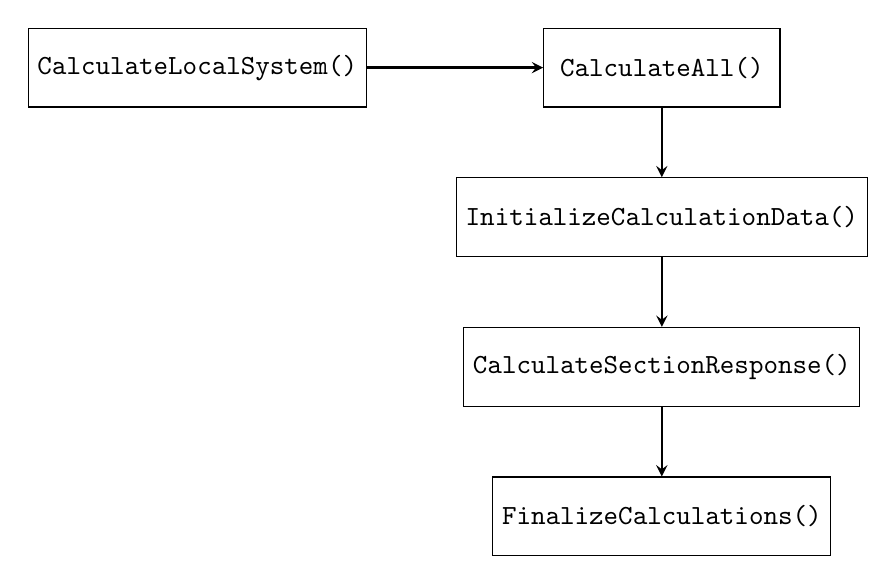
\begin{tikzpicture}[node distance = 1.9cm, auto]
	% Place nodes
	\node [process] (CalculateLocalSystem) {$\texttt{CalculateLocalSystem()}$};
	\node [process, right of=CalculateLocalSystem, xshift = 4cm] (CalculateAll) {$\texttt{CalculateAll()}$};
	\node [process, below of=CalculateAll, xshift = -0cm] (InitializeCalculationData) {$\texttt{InitializeCalculationData()}$};
	\node [process, below of=InitializeCalculationData, yshift = -0cm] (CalculateSectionResponse) {$\texttt{CalculateSectionResponse()}$};
	\node [process, below of=CalculateSectionResponse, yshift = -0cm] (FinalizeCalculations) {$\texttt{FinalizeCalculations()}$};
	% Draw edges
	\draw [arrow] (CalculateLocalSystem) -- (CalculateAll);
	\draw [arrow] (CalculateAll) -- (InitializeCalculationData);
	\draw [arrow] (InitializeCalculationData) -- (CalculateSectionResponse);
	\draw [arrow] (CalculateSectionResponse) -- (FinalizeCalculations);
	\end{tikzpicture}
	\caption{High level overview of DSG element workflow}
	\label{DSGworkflow}
\end{figure}

Initially, the re-implemented virtual method $\texttt{CalculateLocalSystem()}$ is called by the Kratos framework automatically for every $\texttt{ShellThickElement3D3N}$ in the job definition. This method redirects to $\texttt{CalculateAll()}$, which is the main pipeline of the element stiffness calculation, itself calling three key methods: $\texttt{InitializeCalculationData()},$ \break$\texttt{CalculateSectionResponse()}$ and $\texttt{FinalizeCalculations()}$.

Following the general form of the existing shell elements in Kratos, all the data which remains constant through the Gauss Integration loop is calculated beforehand in the function $\texttt{InitializeCalculationData()}$. The DSG element follows this tradition for consistency, although it isn't strictly necessary because it only requires one Gauss point for the numerical integration. Following $\texttt{InitializeCalculationData()}$, $\texttt{CalculateSectionResponse()}$ is called and the material matrix is populated with existing Kratos material classes. It must be noted here that a single 8$\times$8 material matrix $\mathbf{C}$ is returned which is structured as follows (for the setting of 'thick' shell kinematics):

\begin{equation} 
\mathbf{C}_{Kratos} =  
\begin{pmatrix}
	\mathbf{C}_{mem} & \mathbf{0} & \mathbf{0} \\
	\mathbf{0} & \mathbf{C}_{bend} & \mathbf{0} \\
	\mathbf{0} & 	\mathbf{0} & \mathbf{C}_{shear}
\end{pmatrix}
\label{eqtCkratos}
\end{equation} 

At this stage the shear component of the material matrix is unmodified, and is corrected with $\tau$ as per equation \eqref{eqt14}. The DOF arrangement of the material matrix also motivates a slight departure from the strain displacement matrices as presented above. Although the element stiffness matrix can certainly be programmed in it's constitutive parts, as per equation \eqref{eqt5}, it is more concise to calculate it as follows:

\begin{equation} 
\mathbf{K} = \int_A  (\mathbf{B}_{comb}^T \mathbf{C}_{Kratos} \mathbf{B}_{comb} )\ dA
= A\  \mathbf{B}_{comb}^T \mathbf{C}_{Kratos} \mathbf{B}_{comb} 
\label{eqtKkratos}
\end{equation}

A consequence of this arrangement is that the combined strain displacement matrix created in $\texttt{InitializeCalculationData()}$ must conform to the DOF ordering of the material matrix layout.

The element stiffness matrix is calculated according to equation \eqref{eqtKkratos} and subsequently modified to include an artificial drilling DOF stiffness as per equation \eqref{eqtdrilling}. Lastly, this is followed by a call to the Kratos function $\texttt{FinalizeCalculations()}$ which handles the transformation from the element to the global orientation.

The following pseudocode summarises the key calls and operations involved in calculating the DSG element stiffness matrix.

\begin{algorithm}
	\onehalfspacing
	\captionof{algorithm}{DSG triangle element stiffness matrix pseudocode}\label{DSG triangle element stiffness matrix}
	\begin{algorithmic}[1]
		\Require Coordinate transformation instance
		\State \textbf{call} $\texttt{CalculateAll}()$
		\State Resize $LHS$ and $RHS$
		\State \textbf{call} $\texttt{InitializeCalculationData}(data)$
		\State \hspace{\algorithmicindent}Calculate combined strain-displacement matrix $B$
		\State \textbf{call} $\texttt{CalculateSectionResponse}(data)$
		\State \hspace{\algorithmicindent}Retrieve material properties $C$
		\State \hspace{\algorithmicindent}Apply shear stabilization to material matrix $C$
		\State Calculate $LHS$ stiffness matrix
		\State Add in artificial drilling stiffness
		\State Modify $RHS$ residual vector
		\State \textbf{call} $\texttt{FinalizeCalculations}(data,\ displacements,\ LHS,\ RHS)$
		\State \textbf{call} $\texttt{AddBodyForces}(data,\ RHS)$
	\end{algorithmic}
\end{algorithm}


%%%%%%%%%%%%%%%%%%%%%%%%%%%%%%%%%%%%%%%%%%%%%%%%%%%%%%%%%%%%%%%%%%


\section{Mass matrix formulation and implementation}

The mass matrix is necessary to facilitate dynamic analysis with the thick triangular shell element. As per the existing KRATOS shell elements, a lumped mass approach is employed which results in a diagonal mass matrix.

\begin{equation} 
\mathbf{M} =  
\begin{pmatrix}
\mathbf{M}_1 & \mathbf{0} & \mathbf{0}\\
\mathbf{0} & \mathbf{M}_2 & \mathbf{0}\\
\mathbf{0} & \mathbf{0} & \mathbf{M}_3
\end{pmatrix}
\hspace{10mm}
where
\hspace{10mm}
\mathbf{M}_i =  
\begin{pmatrix}
\bar{m} & 0 & 0 & 0 & 0 & 0\\
0 & \bar{m} & 0 & 0 & 0 & 0\\
0 & 0 & \bar{m} &0 & 0 & 0\\
0 & 0 & 0 & 0 & 0 & 0\\
0 & 0 & 0 & 0 & 0 & 0\\
0 & 0 & 0 & 0 & 0 & 0
\end{pmatrix}
\label{eqt15}
\end{equation}

The general lumped mass is determined for a multi-ply material with $n$ plies each of $t_i$ thickness and $\rho_i$ density as follows:

\begin{equation} 
\bar{m} = \frac{A}{3} \sum_{i=1}^n \rho_i t_i
\label{eqt16}
\end{equation}

For a single layer material of area $A$ this reduces to:

\begin{equation} 
\bar{m} = \frac{A}{3} \rho t
\label{eqt17}
\end{equation}

\section{Stress and strain recovery}

While the stiffness and mass matrices enable the calculation of nodal displacements, velocities and accelerations, practical engineering analysis is usually more concerned with the strains and stresses of the structure. The non-zero local strains ($\epsilon_{zz} = 0$) of the 5 parameter element can be arranged in a vector form:

\begin{equation} 
\boldsymbol{\epsilon}^T = \begin{pmatrix}
\boldsymbol{\epsilon}_1 & \boldsymbol{\epsilon}_2 & \boldsymbol{\epsilon}_3
\end{pmatrix}
\hspace{5mm}
with
\hspace{5mm}
\boldsymbol{\epsilon}^T_i = \begin{pmatrix}
\epsilon_{xx} & \epsilon_{xx} & 2\epsilon_{xy} & \epsilon_{xx} & \kappa_{xx} & \kappa_{yy} & 2\kappa_{xy} & 2\epsilon_{xz} & 2\epsilon_{yz}
\end{pmatrix}
\label{eqt18}
\end{equation}

The strain field within the element can be recovered from the displacement field by using the strain displacement matrix, which is constant over the element for the DSG triangle.

\begin{equation} 
\boldsymbol{\epsilon}(\xi,\ \eta) = \mathbf{B}\ \mathbf{u}(\xi,\ \eta)
\label{eqt19}
\end{equation}

In typical finite element programs the strains and stresses are calculated at the Gauss points of the element, which is also how Kratos operates. Since the DSG has one Gauss point in the centre of the element, the strain is recovered from the discrete nodal displacements $\hat{\mathbf{u}}_i$ as follows:

\begin{equation} 
\boldsymbol{\epsilon}_{GP} = \mathbf{B} \sum_{i=1}^{3 nodes} N_i(\xi_{GP},\ \eta_{GP}) \hat{\mathbf{u}}_i
\label{eqt20}
\end{equation}

With the strains determined, the stresses at the Gauss points can be recovered with the material matrix at the Gauss point.

\begin{equation} 
\boldsymbol{\sigma}_{GP} = \mathbf{C}_GP\ \boldsymbol{\epsilon}_{GP}
\label{eqt21}
\end{equation}

The general implementation of the stress and strain recovery described above is illustrated in the following pseudocode.

\begin{algorithm}
	\caption{DSG triangle element stress and strain recovery}
	\label{DSG triangle element stress and strain recovery}
	\begin{algorithmic}[1]
		\Require $requestedQuantity$, calculation of nodal displacements
		\State \textbf{call} $\texttt{InitializeCalculationData}(data)$
		\State \hspace{\algorithmicindent}Calculate strain-displacement matrix $B$
		\State \hspace{\algorithmicindent}Retrieve element $localDisplacements$
		\State $generalizedStrains$ = product$(B,\ localDisplacements)$
		\If{$requestedQuantity$ requires stress} 
				\State \textbf{call} $\texttt{CalculateSectionResponse}(data)$
				\State $generalizedStresses$ = product $(C,\ generalizedStrains)$
				\State Decimal correction of $generalizedStresses$
		\EndIf
		\State Decimal correction of $generalizedStrains$ 
		\If{$requestedQuantity$ requires local orientation} 
				\State Rotate $requestedQuantity$ to local orientation
		\EndIf
		\State Assemble $requestedQuantity$ into $outputMatrix$
		\If{$requestedQuantity$ requires global orientation} 
				\State Rotate $outputMatrix$ to global orientation
		\EndIf
		\State Interpolate $outputMatrix$ to standard Gauss points for visualisation
	\end{algorithmic}
\end{algorithm}